\chapter{Literature Review}
\label{chap2}
In the chapter 1 we have given the introduction of our project, objectives and a thesis break down. Our introduction chapter is giving a complete overview of this project report. This chapter is about the work which is already been done on University Network using Cisco Packet Tracer, and will give a brief details about the articles, papers and literature review.

\section{Literature Review}
This chapter is about studies and literatures that are related to the University Network using Cisco Packet Tracer that the proponents made use of different reading materials (such as thesis, articles, and other web articles) that will help extending the knowledge of the topic. These reading materials will also guide the proponent to improve and develop their proposed system more effectively.

\subsection{Network Topology}
A network topology defines how hosts are connected to a computer network. It
characterizes how the PCs and other hosts are organized, and linked to each other.
\subsubsection{Point to Point Topology}
Point to Point topologies connect two computers together with a single line
connection. The advantage of Point to Point Topology is that it gives a faster connection,
and it is also less expensive than other topologies. The strength of this topology is more
than other kinds of connection\cite{kornilovitch2009fully}.\\
\begin{figure}[H]  %h=positioning
\begin{center}
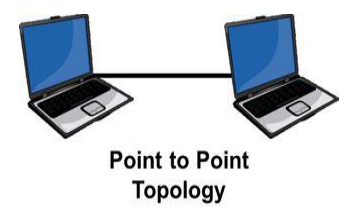
\includegraphics[scale=0.62]{Chapter1/pTopTopology}
\caption{Point to Point Topology}
\label{figure1}
\end{center}
\end{figure}

\subsubsection{Bus Topology}
Bus topology, with the inexpensive configuration, many computers are connected
by a single line of cable. Each side of the main cable must be connected to terminals.
This type of network topology is small and very easy to connect devices together to
making the network. The bus topology uses one main cable for all the connection, and
it�s usually seen in smaller networks. If the main cable is broken, there will be a network
failure such as that seen at a local office level\cite{alsarhan2016computer}.\\

\begin{figure}[H]  %h=positioning
\begin{center}
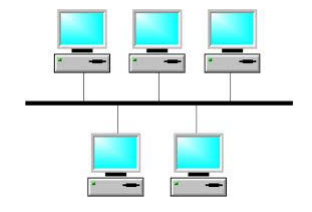
\includegraphics[scale=0.80]{Chapter1/busTopology}
\caption{Bus Topology}
\label{figure1}
\end{center}
\end{figure}

\subsubsection{Ring Topology}
Another topology is the ring topology, which uses a connecting computer in a circle
shape. The source computer sends information to the cable ring, and this information
searches for its destination by accessing each computer on the ring until it gets its
destination node. According to the article ``A review of Network Topology'' by Jiang,
�Adjacent pairs of workstations are directly connected. Other pairs of workstations are
indirectly connected, the data passing through one or more intermediate nodes \cite{jiang2015review}.''
\begin{figure}[H]  %h=positioning
\begin{center}
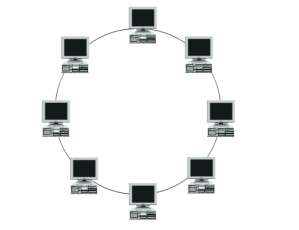
\includegraphics[scale=0.90]{Chapter1/ringTopology}
\caption{Ring Topology}
\label{figure1}
\end{center}
\end{figure}

\subsubsection{Mesh Topology}
The mesh topology requires each computer to be connected directly to multiple
computers, with more than one line connecting all computers to each other. One good
thing about this topology is that if one line fails or cut, it will use the other paths to send
information to the destination. This reduces the probability of a total network failure. 
Mesh topology is faster compared to other kinds of topology, but it is very expensive.
According to the Clarke ``A disadvantage of a mesh topology is the cost of the additional
cabling and network interfaces to create the multiple pathways between each system \cite{clarke2009comptia}.``\\ 
\begin{figure}[H]  %h=positioning
\begin{center}
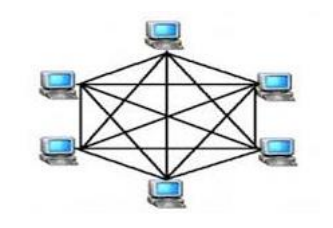
\includegraphics[scale=0.90]{Chapter1/meshTopology}
\caption{Mesh Topology}
\label{figure1}
\end{center}
\end{figure}

\subsubsection{Star Topology}
The star topology is generally used for all networks whereby each device or
computer is connected to a center hub by a direct line. The center hub can be a switch,
router, or server. Each computer connects directly to the center device such as the hub,
router, and server. ``A star topology is designed with each node connected directly to a
central network hub, switch, or concentrator \cite{jiang2015review}.'' It is easy to add
and remove a computer from the network without affecting the network. Pandya, Kartik
mentioned in their article, ``It is easy to replace, install or remove hosts or other devices,
the problem can be easily detected-It is easier to modify or add a new computer without
disturbing the rest of the network by simply running a new line from the computer to the
central location and plugging it to the hub \cite{alsarhan2016computer}.''\\

\begin{figure}[H]  %h=positioning
\begin{center}
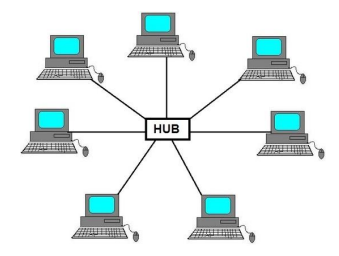
\includegraphics[scale=0.80]{Chapter1/starTopology}
\caption{Star Topology}
\label{figure1}
\end{center}
\end{figure}


%\begin{table}[H]
%%\large
%\centering
%\caption{Consolidated Comparison of all the Systems}
%\label{tab2}
%%begin{adjustwidth}{-2.25in}{Oin}
%
%\begin{tabular}{|c|c|c|c|c|c|}
%\hline  %make a line
%Technology Used&Cost&Feasibility&Reliability&Communication Protocol\\
%\hline %make a line
%GSM&Low&Most Feasible&High&Stable\\
%\hline
%ZigBee&Medium&Small Scale&Low&Least Stable\\
%\hline
%SCADA&High&Not Feasible&High&Stable\\
%\hline
%PLC&Low&Least Feasible&Low&Very Stable\\
%\hline
%WiMAX&Medium&Small Scale&Medium&Stable\\
%\hline
%Mixed&Varies&Feasible&Varies&Varies\\
%\hline
%\end{tabular}
%\end{table}
%
%\small
%\begin{table}[H]
%\caption{Literature Review}
%\label{tab3}
%\centering
%\begin{tabularx}{1\linewidth}{X X X X}
%\toprule
% Paper Reference & Approach & Technology & Accuracy ($\%$) \\
%\toprule
%\cite{khan2020cost}&Cost Benefit Based Analytical Study of AMR and Blind Meter Reading (BMR) used by PESCO(WAPDA)& AMR and BMR &The Blind Meter Reading has internal financial return of about 84 percent while in case of AMR it is 15 percent.\\
%%\toprule
%\hline  %make a line
%\cite{zhao2005research} & Remote Meter Automatic Reading
%Based on Computer Vision & Computer vision techniques & $78\%$\\
%\hline %make a line
%\cite{li2019light} & Light-Weight Spliced Convolution Network-Based
%Automatic Water Meter Reading in Smart City & Network-Based
%Automatic Water Meter Reading & $85.66\%$ \\
%%\toprule
%\hline  %make a line
%\cite{dong2010design} & Wireless AMR System Based on SOPC & SOPC & $59.6\%$ \\
%\hline  %make a line
%\cite{ando2002automatic} & AMR system adopting automatic routing technology & routing technology & $68\%$ \\
%\hline  %make a line
%\cite{wiratama2018gas} & Gas
%billing system based on AMR on diaphragm gas meter with email
%notification & GSM or
%GPRS networks & $79\%$\\
%\hline  %make a line
%\cite{ashna2013gsm} & GSM based automatic AMR system with instant billing & GSM & $88\%$\\
%\hline  %make a line
%\cite{shuo2019digital} & Digital recognition of electric meter with deep learning & Deep Learning Methods & $78\%$\\
%\hline  %make a line
%\end{tabularx}
%\end{table}
%\small
%\begin{table}[H]
%\caption{-- continued from previous Literature Review table \ref{tab3}}
%\label{tab4}
%\centering
%\begin{tabularx}{1\linewidth}{X X X X}
%\toprule
% Paper Reference & Approach & Technology & Accuracy ($\%$) \\
%\toprule
%
%\cite{kulkarni2012gsm} &GSM based AMR system using ARM controller & ARM Controller & $81\%$\\
%\hline  %make a line
%\cite{Ali2012} & Implementation of (AMR) using radio frequency (RF) module & Radio Frequency & $58\%$\\
%\hline  %make a line
%\cite{palaniappan2015automated} & Comparison between different technologies being used in ARM  & GSM, Zigbee, SCADA System, Power Line Communication, WiMAX Technology,  & GSM = $88\%$, Zigbee = $67\%$,SCADA = $63\%$,Power Line = $71\%$,WiMAX = $62\%$,  \\
%\hline %make a line
%\cite{quan2010design} & Design of remote automatic meter reading system based on ZigBee and GPRS & ZigBee and GPRS techniques & $67\%$\\
%\hline  %make a line
%\cite{arun2012design} & Design and implementation of AMR system using GSM, ZIGBEE through GPRS & using GSM, ZIGBEE through GPRS & $89\%$\\
%\hline  %make a line
%\cite{rouf2012neighborhood} & Security and privacy analysis of automatic meter reading systems & Analysises of AMR & -\\
%\hline  %make a line
%\cite{malhotra2013automatic} & AMR and theft control system by using GSM & GSM & $84\%$\\
%\hline  %make a line
%\cite{tan2007automatic} & Automatic power meter reading system using GSM network & GSM network  & $78\%$\\
%\hline  %make a line
%\cite{Jamil2008} & Design and implementation of a wireless AMR system & GSM Network & $86\%$\\
%\hline  %make a line
%\cite{yuan2011remote} & Remote wireless AMR system based on GPRS & GPRS & $88\%$\\
%\hline  %make a line
%\cite{borle2013automatic} & AMR for electricity using power line communication & power line communication & $65\%$\\
%\hline  %make a line
%\end{tabularx}
%\end{table}
%\small
%\begin{table}[H]
%\caption{-- continued from previous Literature Review table \ref{tab4}}
%\label{tab5}
%\centering
%\begin{tabularx}{1\linewidth}{X X X X}
%\toprule
% Paper Reference & Approach & Technology & Accuracy ($\%$) \\
%\toprule
%\cite{mlakic2017designing} & Designing AMR system using open source hardware and software &open source hardware and software & $59\%$\\
%\hline  %make a line
%\cite{khalifa2010survey} & A survey of communication protocols for auto-
%matic meter reading applications, & Communication Protocols & - \\
%\hline
%\bottomrule
%\end{tabularx}
%\end{table}

%\section{Concluding Remarks}
%In this chapter, we have given a overall review about the literature related to Speech Processing Using MATLAB. MATLAB is a programming and numeric computing platform used by millions of engineers and scientists to analyze data, develop algorithms, and create models.\\\\
%In the chapter 3 we will proposed methodology which we will use for our project with block diagrams, flowcharts, Mathematical Modeling, escudo code and component selection related to the hardware and software.

